\documentclass[conference]{IEEEtran}
%=====PACKAGES=====
\usepackage{amsmath,amssymb}		%To use math symbols
\usepackage{graphicx}				%To include figures
\usepackage[font=footnotesize]{caption}	%To specify the font of captions
\usepackage{url}
\usepackage{graphicx}


%=====SYMBOLS DEFINITIONS=====
\def \R{\mathbb{R}}
\def \X{\boldsymbol{\rm X}}
\def \y{\boldsymbol{\rm y}}
\def \bbeta{\boldsymbol{\beta}}
\def \T{\mathsf{T}}


%=====DOCUMENT=====
\begin{document}
\title{Antibiotic Resistance Classification}
\author{
\IEEEauthorblockN
{Hasin Yeahia | Mark Lynch | Samir Vyas \\
\textit{Georgia State University}}

\IEEEauthorblockA{\sc{CS 4780 Final Project}}
}
\maketitle

%=====ABSTRACT=====
\begin{abstract}
\begin{center}
The goal is to classify the effects of antiobiotics to either carbenicillan or
tobramycin on a given bacteria set. Initially, we normalized a given excel dataset and determined a threshold of fifty or greater to be resistant and if 49 and below to be anti-resistant. We then decided to desaturate and convert the images to grayscale and then downsize the large images into something more
manageable. The images are then stratified into arrays of values and split into layers by a python package named Keras. Next, we train our model by feeding in the edited images and letting the model adapt and learn what feature sets it should be internalizing. Finally we let the model get fed a folder of testing data that has been removed from the original image dataset. The end result of which is a marked percentage indicating an accuracy of our model. 
\end{center}

\end{abstract}



%=====INTRODUCTION=====
\section{Introduction}
\label{secName}
The report will be explaining our unique approach at a classification problem. The primary goal is to determine and categorize our given bacteria image set and determine the effects of the antibiotics carbenicillan and tobramycin. The categorization of this would fall under neural networks - specifically convolution neural networks. Convolutional networks rely on vectorized images and layering techniques which in our case is supplied by the keras package for python. Our initial approach was to convert all the training data into greyscale. Next, we split the images into arrays of pixel values which are placed into layers. These layers are then formed together to be trained by our model to interpret and classify an image. The model itself has a parameter indicating a split between training data and testing data, which in our case was an 85 - 15 split.


%=====DATA=====
\section{Data}
Our initial approach was to breakdown and understand the tables given in the initial excel document. We normalized the given values into 0 to 100, as shown below: 
\begin{table}[h]
\begin{center}
\begin{tabular}{| c | c | c | c | c |}
\hline
Image & Carb & Toby & CNormalized & TNormalized\\ \hline \hline
PIL-1\_3dayLBCR-1 & 19 & 4 & 0 & 37.5\\ \hline
PIL-1\_3dayLBCR-2 & 19 & 4 & 0 & 37.5\\ \hline
\vdots & \vdots & \vdots & \vdots & \vdots\\ \hline
PIL-78\_3dayLBCR-1 & 30 & 6 & 100 & 27.5\\ \hline
\end{tabular}
\caption{Before and After Normalization of Values}
\label{tabDeliverable}
\end{center}
\end{table}


This method of preprocessing the excel data columns for carb and toby more clearly defined the relationship between the two in the image dataset. We also made a choice to determine an arbritrary yet sensible threshold value of 50; the dividing line of 50 seems appropriate given a value range between 0 and 100.

%=====METHODS=====
\section{Methods}
Our approach had to be utilized by a programming language that seemed as a best fit for our objective. Matlab and R are viable options but we noticed that the best support with the most documentation was with python. Our approach could not be done with simple importing and user defined methods; we required higher level functionality from specific libraries to achieve our goals. Python can handle a variety of functionalities depending on what libraries and packages are utilized. 

Our primary focus was on tensorflow and keras. Our initial goal was to identify any and all missing and incomplete entries in the excel document that outlines the effects of the stated antibiotics. After removing any missing or incorrectly labeled images, we had a clean base to work with.

Our next tactic was to convert the images to greyscale. This reduces the amount of complexity and reduces parameters when it comes to comparisons and training the model. Anything that can reduce unnecessary complexity sharpens our focus and removes any possible mishaps or misteps. 


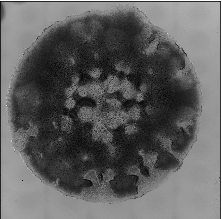
\includegraphics{gray.jpg} 


We then created a convolutional layer which requires an input of consistent image width, height, depth and number of images. This layer involved a concept called pooling where local clusters of specified small pixel groupings are formed to create a clustering of layers. These layers are then outlayed in an array of values which are then used to generate comparisons. 

The next step in the procedure is to train the model. This requires the images to be preprocessed and following specified parameters so the model can truly digest and properly understand the dataset it needs to learn to finally move onto the testing state.

The key culmination of all prior steps is the testing stage. The testing stage is handled internally as one of the parameters in keras is validation-split. This is the fraction of data utilized as testing data. Testing data inherently implies that the model has not seen the or become familiar with that specific grouping of images. This is important as the whole premise is for the model to recognize similaries based off of matrix array comparisons and returns an accuracy reading that is much higher than a coin toss reading, i.e a properly trained model should be able to guess and ascertain the proper category of the testing image.

We felt a need to bolster certain image groups, i.e carbenicillinResistant as those images were fewer in comparison to others. Smaller datasets typically have a lower chance of being effective in comparison to larger datasets since the more epochs a model can train the stronger the generated accuracy. That logic was not applied to all groups of images so in the end they were removed. 

%=====EXPERIMENTS=====
\section{Experiments}
There were several parameters that were fine-tuned and experimented upon. Take our batch-size for example. These values determine the number of samples to work through before updating our internal model. We experimented with values 8, 16 and 32. The highest performance with the best accurarcy was duly noted at a batch size of 16. 

Another parameter under keras is the epoch which is best explained as total passes through the entire imported image dataset. This value allows the model to continously pass through the dataset and approach a plateau which indicates no more "learning" can be achieved. We achieved this around 75 epochs, although the general convergence can be given as a range between 50 to 60.

Accuracy is the entire premise of this report. We had several hurdles regarding accuracy being quite low; initially our model was outputting around 50\% which can be labeled as a simple coin-toss: essentially worthless. Through various manipulations of specific parameters, we achieved a steady result of between 75-80\%. This number is a strict reflection of the model reading over the test images. Our definied validation-split of 85 and 15; generally, an 80-20 split is sufficient but given that our total image data set is considered small, we wanted our model to train with the most amount of data possible. However, there needs to be sufficient testing data as well which is how we settled upon an 85-15 split.

Furthermore we came to a conclusive reading of the testing data files and proceeded to export the values as a csv. 


%=====CONCLUSIONS=====
\section{Conclusions}
Our results were heavily influenced by a couple factors outside of our control. The accuracy of our results were lower than expected since our working image dataset is generally considered to be small. Larger datasets allow training models to become more fleshed out and accurate by allowing the model to train upon a wider volume of varied data. Our results are also hindered by our brief experience with machine learning technologies. Experience and prior projects would be typically beneficial when dealing with high level problem sets such as image categorization. 

The results are being generated by running the entire test data through the models we created. Our results are best explained by the below chart.

\begin{table}[h]
\begin{center}
\begin{tabular}{| c | c | c |}
\hline
Image & Prediction 1 & Prediction 2 \\ \hline \hline
PIL-1\_3dayLBCR-1 & tobyNotRes & carbRes \\ \hline
PIL-1\_3dayLBCR-2 & tobyNotRes & carbRes \\ \hline
\vdots & \vdots & \vdots \\ \hline
PIL-86\_3dayLBCR-3 & tobyRes & carbNotRes \\ \hline
PIL-9\_3dayLBCR-4 & tobyNotRes & carbRes \\ \hline
PIL-90\_3dayLBCR-4 & tobyRes  & carbNotRes \\ \hline
PIL-94\_3dayLBCR-4 & tobyNotRes & carbNotRes \\ \hline
\end{tabular}
\caption{Snippet of Images and corresponding labels}
\label{tabDeliverable}
\end{center}
\end{table}

The categorization of Res and NotRes is defined as either resistant or not resistant. 

\begin{table}[h]
\begin{center}
\begin{tabular}{| c | c | c |}
\hline
Method & Toby & Carb \\ \hline \hline
Convolutional NN & 82.26\% & {74.24\%} \\ \hline

\end{tabular}
\caption{Predictions via Convolutional Neural Network.}
\label{tabSummary}
\end{center}
\end{table}

After much testing with various parameters regarding the codebase, we approached a steady plateau for an accuracy where it was at it's maximum. If given a larger dataset we believe our model would have been trained and learned more optimally. The given output at that point would be hypothetically a higher accuracy reading. 

Given that batch data generated by laboratories are typically several hundred if not several thousand image data files, manual categorization of said data is highly inefficient. This dataset would require quick processing and categorization. A variety of methodologies would be necessary to determine the highest efficiency and highest accuracy but given the scope and time frame of this project we had to narrow our scope down to one classification method: convolutional neural networks.  
We believe that convolutional neural networks are a satisfactory method to analyzing bacteria datasets. 

%=====REFERENCES=====
\begin{thebibliography}{1}

\bibitem{StackOverflow}
Various troubleshooting | StackOverflow[online]
Available at: https://stackoverflow.com/ [April 2019].

\bibitem{DataExchange}
Various machine learning | DataExchange[online]
Available at: https://datascience.stackexchange.com/ [April 2019].

\bibitem{TensorFlow}
Learn and use machine learning  |  TensorFlow Core  |  TensorFlow. [online] Available at: https://www.tensorflow.org/tutorials/keras [April 2019].

\bibitem{Project}
Group Project Github | Hasin | Mark | Samir [online]
Available at: https://github.com/hasinyeahia/Fundamentals [April 2019]

\end{thebibliography}

\end{document}


